\documentclass[a4paper,18pt,twoside]{report}
\usepackage[french]{babel}
\usepackage[T1]{fontenc}
\usepackage[utf8]{inputenc}
\usepackage{geometry}
\geometry{hmargin=2.5cm,vmargin=1.5cm}
\usepackage{graphicx}
\usepackage[urlcolor=blue,linkcolor=black,colorlinks=true]{hyperref}
\usepackage{listings}
\usepackage{color}
\usepackage{verbatim}
\usepackage{shadethm}


\definecolor{green}{rgb}{0,0.6,0}
\begin{comment}pour trouver la couleur en décimal, on divise la valeur de RGB par 255. Exemple, si RGB(15,150,144), faire RGB(15/255,150/255,144/255)
\end{comment}
\definecolor{gray}{rgb}{0.5,0.5,0.5}
\definecolor{mauve}{rgb}{0.58,0,0.82}
\definecolor{orange}{rgb}{0.90,0.45,0}
\definecolor{grey}{rgb}{0.79,0.79,0.80}

%------------------------------------------------------------------
% Réglages pour le code source du langage C
\lstdefinestyle{customc}{
	belowcaptionskip=1\baselineskip,
	breaklines=true,
	frame=L,
	xleftmargin=\parindent,
	language=C,
	showstringspaces=false,
	basicstyle=\footnotesize\ttfamily,
	keywordstyle=\bfseries\color{green},
	commentstyle=\itshape\color{mauve},
	identifierstyle=\color{blue},
	stringstyle=\color{orange},
}

\lstdefinestyle{customasm}{
	belowcaptionskip=1\baselineskip,
	frame=L,
	xleftmargin=\parindent,
	language=[x86masm]Assembler,
	basicstyle=\footnotesize\ttfamily,
	commentstyle=\itshape\color{purple!40!black},
}

\lstset{escapechar=@,style=customc}
%-----------------------------------------------------------------------


\title{Traduction de C++ Primer 5th Edition}
\author{Auteurs: Stanley B. Lippman, Josée Lajoie et Barbara E. Moo}
\date{Traduction non-officielle: Stomab}


\begin{document}

\begin{titlepage}

	\textsc{\LARGE C++ Primer 5th Edition}

\end{titlepage}
\maketitle

\tableofcontents


\newpage

\section{Préface}
De nombreux programmeurs ont appris le C++ avec les précédentes éditions de \textit{C++ Primer}. Pendant ce temps, le C++ a gagné en maturité: son objectif, encouragé par la communauté de développeurs, a été de se focaliser davantage sur l'efficacité du \textit{programmeur} plutôt que de l'efficacité de la \textit{machine}.

En 2011, le comité des normes C++ a publié une révision majeure de la norme ISO C++. Cette révision est la dernière étape de l'évolution du C++ et continue de mettre l'accent sur l'efficacité du programmeur. Les principaux objectifs de la nouvelle norme sont les suivants:

\medbreak
\begin{itemize}
	\item[\textbullet] Rendre le langage plus uniforme, plus facile à enseigner et à apprendre ;
	\item[\textbullet] Simplifier les bibliothèques standards, les rendre plus sûres et plus efficaces à utiliser ;
	\item[\textbullet] Faciliter l'écriture des abstractions et des bibliothèques de manière efficace.
\end{itemize}

\medbreak
Dans cette édition, nous avons intégralement revu le \textit{C++ Primer} en y incorporant les dernières normes. Vous pourrez apprécier les différents changements impactés par ces nouvelles normes en consultant la table des matières.

Certains ajouts dans la nouvelle norme, tels que \textit{auto} pour l'inférence de type, sont omniprésents. Ces fonctionnalités rendent le code de cette édition plus facile à lire et à comprendre. Les programmes (et les programmeurs !) peuvent ignorer ces détails, pour pouvoir se concentrer sur ce que le programme est censé faire. D'autres nouvelles fonctionnalités, telles que les pointeurs intelligents et les conteneurs avec éléments déplacés, permettront d'écrire des classes plus sophistiquées sans avoir à composer avec les complexités de la gestion des ressources. En conséquence, vous pourrez apprendre à écrire vos propres classes bien plus tôt dans le livre par rapport à l'édition précédente.

Nous avons mis en évidence, dans le texte, les nouvelles fonctionnalités de la dernière norme, à l'aide d'une icône spécifique. Nous espérons que les lecteurs connaissant déjà le C++, trouveront ces remarques pertinentes pour décider où concentrer leur attention. \marginpar{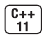
\includegraphics{images/cpp11.jpg}}Nous espérons également que ces remarques, encadrées par ces icônes spécifiques, aideront à expliquer les messages d'erreur des compilateurs qui pourraient ne pas encore prendre en charge toutes les nouvelles fonctionnalités. Bien que la quasi-totalité des exemples de ce livre ont été compilés avec une version récente du compilateur GNU, nous sommes conscients que certains lecteurs n'auront pas encore accès à des compilateurs récents et mis à jour. Même si de nombreuses fonctionnalités ont été ajoutées pour répondre aux nouvelles normes, le langage de base reste inchangé et constitue l'essentiel du matériel que nous couvrons. Les lecteurs peuvent utiliser ces icônes pour noter quelles fonctionnalités peuvent ne pas être encore disponibles avec leur compilateur.

\subsection{Pourquoi lire cet ouvrage ?}
Le C++ moderne peut se résumer en trois parties :

\medbreak
\begin{itemize}
	\item[\textbullet] Un langage de bas niveau, dont une grande partie est héritée du C ;
	\item[\textbullet] Des fonctionnalités de langage plus avancées qui nous permettent de définir nos propres types et organiser des programmes et des systèmes à grande échelle ;
	\item[\textbullet] La bibliothèque standard, qui utilise ces fonctionnalités avancées pour fournir des structures de données et des algorithmes.
\end{itemize}

\medbreak
La plupart des ouvrages présentent le C++ dans l'ordre dans lequel il a évolué. Le sous-ensemble C est d'abord enseigné, puis viennent les fonctionnalités les plus abstraites de C++ sous forme de sujets avancés à la fin du livre seulement. Il y a deux problèmes avec cette approche: les lecteurs peuvent s'enliser dans les détails inhérents à la programmation de bas niveau et abandonner par frustration. Ceux qui persévèrent prennent de mauvaises habitudes qu'ils doivent désapprendre plus tard.

Nous adoptons la démarche inverse: dès le début, nous utilisons les fonctionnalités qui permettent aux programmeurs d'ignorer les détails inhérents à la programmation de bas niveau. Par exemple, nous introduisons et utilisons les bibliothèques \textit{string} et \textit{vector} avec les opérateurs arithmétiques et les tableaux. Les programmes qui utilisent ces types de bibliothèques sont plus faciles à écrire, plus facile à comprendre, et moins sujets aux erreurs.

Trop souvent, la bibliothèque est enseignée comme un sujet avancé. Au lieu d'utiliser la bibliothèque, de nombreux livres utilisent des techniques de programmation de bas niveau basées sur des pointeurs vers des tableaux de caractères et une gestion dynamique de la mémoire. Obtenir des programmes qui utilisent ces techniques de bas niveau pour fonctionner correctement est beaucoup plus difficile que d'écrire le code C++ correspondant à l'aide de la bibliothèque.

Tout au long de \textit{C++ Primer}, nous mettons l'accent sur le bon style à adopter: nous voulons vous aider, le lecteur, à acquérir immédiatement de bonnes habitudes et à éviter d'avoir à désapprendre de mauvaises habitudes à mesure que vous apprenez de nouvelles choses de plus en plus complexes. Nous soulignons les questions particulièrement délicates et mettons en garde contre les idées fausses et les pièges courants.

Nous expliquons également la raison d'être des règles, sans nous contenter de les décrire, mais en expliquant également le pourquoi de leur existence. Nous croyons qu'en comprenant pourquoi les choses fonctionnent ainsi, les lecteurs peuvent faciliter plus rapidement leur compréhension du langage.

Même si vous n'avez pas spécialement besoin de connaître le C pour comprendre ce livre, nous supposons que vous en savez suffisamment sur la programmation pour écrire, compiler et exécuter un programme dans un langage moderne structuré en blocs. En particulier, nous partons du principe que vous savez utiliser des variables, écrire et appeler des fonctions et que vous avez déjà utilisé un compilateur. 

\subsection{Ce qui change dans cette nouvelle édition}
La nouveauté de cette édition de \textit{C++ Primer} est l'ajout d'icônes dans les marges pour guider le lecteur. C++ est un langage puissant qui offre des fonctionnalités adaptées à des raisonnements particuliers de programmation. Certaines de ces fonctionnalités sont très importantes pour les grandes équipes de projet, mais peuvent ne pas être nécessaires pour de plus petits projets. Par conséquent, tous les programmeurs ne sont pas dans l'obligation de connaître chaque détail de chaque fonctionnalité. Nous avons ajouté ces icônes accessoires pour guider le lecteur et lui indiquer les parties qui peuvent être approfondies ultérieurement ou au contraire, les sujets qui sont plus essentiels.

\reversemarginpar{
\includegraphics{images/livre.jpg}}Certains passages du livre qui abordent les principes fondamentaux du langage, seront signalés par une image représentant une personne plongée dans un livre. Les sujets traités dans les sections marquées de cette manière forment la partie centrale du langage. Tout le monde devrait lire et comprendre ces passages du livre.

Nous avons également indiqué les passages qui couvrent des sujets avancés ou à usage spécifique. Ces sections peuvent être sautées ou survolées lors d'une première lecture. Nous indiquons les passages en question à l'aide d'une icône représentant une pile de livres.\marginpar{
\includegraphics{images/pile.png}} Cela signifie que vous pouvez poser le livre en toute sécurité à ce stade de la lecture. Parcourir ces différentes sections peut s'avérer utile pour se tenir informé de ce qu'il est possible de faire. Cependant, il n'y a aucune raison de passer du temps à étudier ces sujets jusqu'à ce que vous ayez réellement besoin d'utiliser la fonctionnalité dans vos propres programmes.

Pour aider les lecteurs à retenir leur attention sur un passage en particulier, nous avons mis en évidence les concepts particulièrement délicats avec une icône en forme de loupe. Nous espérons que les lecteurs prendront le temps de bien comprendre le sujet traité dans les passages marqués ainsi. \marginpar{
\includegraphics{images/loupe.png}}Dans au moins certaines de ces sections, l'importance du sujet peut ne pas être évidente ; mais nous misons sur votre capacité à comprendre l'importance des sujets abordés et qui s'avèrent essentiels à la compréhension du langage.

Ce qui reste inchangé, c'est que \textit{C++ Primer} est un guide didactique clair, correct et complet sur C++. Nous enseignons le langage en présentant une série d'exemples de plus en plus sophistiqués, qui expliquent les fonctionnalités du langage et montrent comment tirer le meilleur parti de C++.

\subsection{Structure de ce livre}
Nous commençons par couvrir ensemble les bases du langage et de la bibliothèque dans les parties I et II. Ces parties couvrent suffisamment de contenu pour vous permettre d'écrire des programmes. La plupart des programmeurs en C++ ont besoin de connaître essentiellement tout ce qui sera abordé dans cette partie du livre.

En plus d'enseigner les bases du C++, le contenu des parties I et II vise un autre objectif important: en utilisant les fonctions définies par la bibliothèque, vous deviendrez plus à l'aide avec l'utilisation de techniques de programmation de haut niveau. Les fonctionnalités de la bibliothèque sont elles-mêmes des types de données abstraites qui sont généralement écrites en C++. La bibliothèque peut être définie en utilisant les mêmes caractéristiques de construction de classe que ...

\bigbreak
[A CONTINUER - INCOMPLET]

\chapter{COMMENCER}

Ce chapitre introduit la plupart des éléments de base de C++: types, variables, expressions, déclarations, et les fonctions. En cours de route, nous expliquerons brièvement comment compiler et exécuter un programme.

Après avoir lu ce chapitre et réalisé les différents exercices, vous devriez être capable d'écrire, de compiler et d'exécuter des programmes simples. Les chapitres suivants partiront du principe que vous pouvez utiliser les fonctionnalités présentées dans ce chapitre et expliqueront ces fonctionnalités plus en détail.

\newpage
\textbf{Le secret de la réussite} dans l'apprentissage d'un nouveau langage de programmation est d'écrire des programmes. Dans ce chapitre, nous allons écrire un programme pour résoudre un problème simple pour une librairie. Notre magasin conserve un fichier de transactions ; chacune d'elles enregistrant la vente d'un ou plusieurs exemplaires d'un même livre. Chaque transaction contient trois éléments de données:

\medbreak
\begin{lstlisting}[language=C]
	0-201-70353-X 4 24.99
\end{lstlisting}
\medbreak
Le premier élément est un numéro ISBN (International Standard Book NUmber, l'identifiant unique d'un livre), le second est le nombre de copies qui ont été vendues, et le dernier est le prix auquel chacun de ces exemplaires a été vendu. De temps en temps, le propriétaire de la librairie lit ce fichier et pour chaque livre calcule le nombre d'exemplaires vendus, le revenu total de ce livre et le prix de vente moyen.

Pour pouvoir réaliser ce programme, nous devons parcourir quelques fonctionnalités de base du C++. De plus, nous allons avoir besoin de savoir comment compiler et exécuter un programme.

Bien que nous n'ayons pas encore conçu notre programme, il est facile de deviner que l'on va devoir :

\medbreak
\begin{itemize}
	\item[\textbullet] Définir des variables ;
	\item[\textbullet] Faire l'entrée et la sortie ;
	\item[\textbullet] Utiliser une structure de données qui contiendra les données ;
	\item[\textbullet] Tester si deux enregistrements ont le même ISBN ;
	\item[\textbullet] Créer une boucle qui traitera chaque enregistrement du ficher de transaction.
\end{itemize}
 
\medbreak
Nous allons commencer à nous intéresser à la résolution de ces sous-problèmes en C++, puis nous écrirons notre programme de gestion de librairie.

\section{Écrire un programme simple en C++}
Chaque programme en C++ contient une ou plusieurs \textbf{fonctions}, dont l'une d'entre elles doit être appelée \textbf{main}. Le système d'exploitation exécute un programme C++ en appelant \textit{main}. Voici la syntaxe de base d'une fonction \textit{main} qui pour l'instant ne fait rien, mais renvoie une valeur au système d'exploitation:

\medbreak
\begin{lstlisting}[language=C]
	int main()
	{
		return 0;
	}
\end{lstlisting}
\medbreak

Une définition de fonction comporte quatre éléments: un \textbf{type de valeur renvoyée}, le \textbf{nom de la fonction}, une \textbf{liste de paramètres} (éventuellement vide) entre parenthèses, et le \textbf{corps de la fonction}. Bien que \textit{main} est un peu particulière à certains égards, nous la définissons de la même manière que toute autre fonction.

Dans cet exemple, \textit{main} ne dispose que d'une liste vide de paramètres (indiquée par les parenthèses () qui ne contiennent rien à l'intérieur). Dans la partie 6.2.5 de livre, nous verrons les autres types de paramètres que nous pouvons définir pour la fonction \textit{main}.

La dernière partie d'une définition de fonction, le corps de la fonction, est un \textbf{bloc d'instructions} qui commence par une accolade ouvrante et se termine par une accolade fermante:

\medbreak
\begin{lstlisting}[language=C]
	{
		return 0;
	}
\end{lstlisting}
\medbreak

La seule instruction de ce bloc est \textit{return}, qui est donc l'instruction qui termine la fonction. Comme c'est le cas ici, un \textit{return} peut également renvoyer une valeur à l'appelant de la fonction. Lorsqu'un \textit{return} inclut une valeur, cette valeur renvoyée doit avoir un type compatible avec le type déclaré dans la fonction. Dans cette exemple, le type de retour de \textit{main} est \textit{int} et la valeur retournée est 0, qui donc est un \textit{int}.

\begin{shadebox}Notez le point-virgule à la fin de l'instruction \textit{return}. Les points-virgules marquent la fin de la plupart des instructions en C++. On peut facilement les oublier ce qui conduit à de mystérieux messages d'erreur du compilateur.
\end{shadebox}

Sur la plupart des systèmes, la valeur renvoyée par \textit{main} est un indicateur d'état. Un 0 retourné indique un succès. Un retour différent de zéro a une signification qui est définie par le système. Habituellement, un retour différent de zéro indique le type d'erreur qui s'est produit.

\begin{shadebox}
\textbf{NOTION CLÉ: LES TYPES}

Les types sont l'un des concepts les plus fondamentaux de la programmation et un concept sur lequel nous reviendrons encore et encore dans ce livre. Un type définit à la fois le contenu d'une donnée et les opérations possibles sur cette donnée.

Les données manipulées par nos programmes sont stockées dans des variables et chacune a un type. Lorsque le type d'une variable nommée \textit{v} est \textit{t}, on dit souvent que "v a le type de t" ou, indifféremment, que "v est un t".

\end{shadebox}

\subsection{Compilation et Exécution de Notre Programme}
Après avoir écrit le programme, nous devons le compiler. Comment compiler un programme dépend de votre système d'exploitation et de votre compilateur. Pour plus de détails sur la manière dont votre compilateur fonctionne, consultez le manuel de référence ou demandez à un collègue compétent.

De nombreux compilateurs basés sur PC sont exécutés à partir d'un environnement de développement intégré (IDE). Il s'agit d'un package qui contient : le compilateur et des outils de construction et d'analyse. Ces IDE peuvent être un atout majeur dans le développement de programmes volumineux, mais nécessite un peu de temps pour apprendre à les utiliser efficacement. Apprendre à utiliser de tels environnements dépasse largement le cadre de ce livre.

La plupart des compilateurs, y compris ceux fournis avec un IDE, fournissent une interface en ligne de commande. À moins que ne connaissiez déjà l'IDE, vous trouverez peut-être plus facile de démarrer avec l'interface de ligne de commande. Cela vous permettra de vous concentrer sur l'apprentissage C++ d'abord. De plus, une fois que vous comprenez le langage, l'IDE est susceptible d'être plus facile à apprendre.

\subsubsection{Convention pour les noms de fichier source du programme}

Que vous utilisiez une interface en ligne de commande ou un IDE, la plupart des compilateurs s'attendent à ce que le code source du programme soit stocké dans un ou plusieurs fichiers. Ces fichiers sont appelés: \textbf{les fichiers sources}. Sur la plupart des systèmes, le nom d'un fichier source se termine par une extension, c'est à dire un point suivi de plusieurs caractères. L'extension indique au système que le fichier est un programme C++. Les compilateurs ont adopté certaines conventions au niveau de l'extension. Ainsi, on retrouve habituellement les extensions \textit{.cc}, \textit{.cxx}, \textit{.cpp}, \textit{.cp} et \textit{.C}.

\subsubsection{Utiliser le compilateur en ligne de commande}

Si nous utilisons une interface en ligne de commande, nous compilerons généralement un programme dans une fenêtre de console (tel qu'un terminal shell sur un système UNIX ou l'invite de commande pour Windows). Supposons que notre programme principal soit écrit dans un fichier nommé \textit{prog1.cc}, nous pourrions le compiler en utilisant une commande telle que :

\medbreak
\begin{lstlisting}[language=C]
	$ CC prog1.cc
\end{lstlisting}
\medbreak

où CC nomme le compilateur et \$ est le prompt du terminal. Le compilateur génère un fichier exécutable. Sur Windows, ce fichier exécutable est nommé \textit{prog1.exe}. Les compilateurs UNIX ont tendance à placer leurs exécutables dans des fichiers nommés \textit{a.out}.

Pour lancer cet exécutable sur Windows, il suffit d'écrire le nom de celui sans être obligé de préciser l'extension \textit{.exe} :

\medbreak
\begin{lstlisting}[language=C]
	$ prog1
\end{lstlisting}
\medbreak

Sur certains systèmes, vous devez spécifier explicitement l'emplacement du fichier, même si le fichier est dans le répertoire ou le dossier en cours. Dans ce cas, on écrirait :

\medbreak
\begin{lstlisting}[language=C]
	$ .\prog1
\end{lstlisting}
\medbreak

Le point "." qui précède l'antislash indique que le fichier se trouve dans le répertoire courant.

Pour lancer un exécutable sous UNIX, nous utilisons le nom complet du fichier, y compris l'extension :

\medbreak
\begin{lstlisting}[language=C]
	$ ./a.out
\end{lstlisting}
\medbreak

La valeur renvoyée par \textit{main} est accessible de manière dépendante du système. Sur systèmes UNIX et Windows, après avoir exécuté le programme, vous devez émettre une commande \textit{echo} appropriée.

Sur les systèmes UNIX, on obtient le statut en écrivant :

\medbreak
\begin{lstlisting}[language=C]
	$ echo $?
\end{lstlisting}
\medbreak

Pour obtenir le statut sur Windows, on écrit :

\medbreak
\begin{lstlisting}[language=C]
	$ echo %ERRORLEVEL%
\end{lstlisting}
\medbreak

\begin{shadebox}
	\textbf{LANCER LE COMPILATEUR GNU OU MICROSOFT}
	
	La commande utilisée pour lancer le compilateur C++ varie selon les compilateurs et les systèmes d'exploitation. Les compilateurs les plus courants sont le compilateur GNU et le compilateur Microsoft Visual Studio.Par défaut, la commande pour exécuter le compilateur GNU est \textbf{g++}:
	
	\medbreak
	\begin{lstlisting}[language=C]
		$ g++ -o prog1 prog1.cc
	\end{lstlisting}
	\medbreak
	
	Le symbole \$ est le prompt. Le \textbf{-o prog1} est un argument pour le compilateur et il nomme le fichier dans lequel sera mis le fichier exécutable. La commande génère un fichier exécutable nommé \textbf{prog1} ou \textbf{prog1.exe}, en fonction du système d'exploitation. Sur UNIX, les fichiers exécutables n'ont pas d'extension ; sur Windows, l'extension est \textbf{.exe}. Si l'on n'avait pas mis le \textbf{-o prog1}, le compilateur aurait généré un exécutable appelé \textbf{a.out} sur un système UNIX et \textbf{a.exe} sur Windows. (À noter : selon la version du compilateur GNU que vous utilisez, vous devrez peut-être spécifier \textbf{-std=c++0x} pour activer la prise en charge de C++ 11).   
	
	La commande pour lancer le compilateur Microsoft Visual Studio 2010 est \textbf{cl}:
	
	\medbreak
	\begin{lstlisting}[language=C]
		$ C:\Users\me\Programs> cl /EHsc prog1.cpp
	\end{lstlisting}
	\medbreak
	
	Ici : \textbf{C:/Users/me/Programs>} est le prompt du système et \textbf{/Users/me/Programs} est le nom du répertoire courant (alias: le dossier courant). La commande \textbf{cl} invoque le compilateur, et \textbf{/EHsc} est l'option du compilateur qui active la gestion standard des exceptions. Le compilateur Microsoft génère automatiquement un exécutable avec un nom qui correspond au premier nom du fichier source. L'exécutable a l'extension \textbf{.exe} et le même nom que le fichier source. Dans notre cas, l'exécutable est nommé \textbf{prog1.exe}.
	
	Les compilateurs incluent généralement des options pour générer des avertissements sur constructions problématiques. C'est généralement une bonne idée d'utiliser ces options. Notre préférence est d'utiliser \textbf{-Wall} avec le compilateur GNU, et utiliser \textbf{/W4} avec les compilateurs Microsoft.
	
	Pour plus d'informations, consultez le guide utilisateur de votre compilateur.
	
\end{shadebox} 

\textbf{EXERCICES SECTION 1.1.1}
\begin{shadebox}
	
	\textbf{Exercice 1.1: }Passez en revue la documentation de votre compilateur et déterminez quelle convention de nommage de fichier il utilise.
	
	\textbf{Exercice 1.2: }Modifiez le programme pour retournez \textbf{-1}. Une valeur de retour -1 est souvent traitée comme un indicateur que le programme a échoué. Recompilez et exécutez votre programme pour voir comment votre système traite une indication de panne du \textit{main}.
\end{shadebox} 

\section{Un premier regard sur les Entrées/Sorties}

Le langage C++ ne définit aucune instruction pour effectuer une entrée ou une sortie (Input/Output).Au lieu de cela, le C++ inclut une bibliothèque standard étendue qui fournit des IO (et de nombreuses autres fonctionnalités).Pour de nombreuses raisons, y compris les exemples de ce livre, il suffit de connaître quelques concepts et opérations de base de la bibliothèque IO.

La plupart des exemples de ce livre utilisent la bibliothèque \textbf{iostream}. Deux types de noms sont des fondamentaux de la bibliothèque \textit{iostream} \textbf{istream} et \textbf{ostream}, qui représentent les flux d'entrée et de sortie. Un flux est une séquence de caractères lus ou écrits sur un périphérique IO. Le terme \textit{flux} est utilisé pour suggérer l'idée que les caractères sont générés, ou consommés, séquentiellement dans le temps.

\subsubsection{Objets d'entrée et de sortie standard}
La bibliothèque définit quatre objets. Pour gérer l'entrée, nous utilisons un objet de type \textit{istream} appelé \textbf{cin} (prononcé ci-in). Cet objet est également appelé \textbf{standard input}. Pour la sortie, nous utilisons un objet \textit{ostream} appelé \textbf{cout} (prononcé ci-out). Cet objet est connu comme le \textbf{standard output}. La bibliothèque définit deux autres objets \textit{ostream}, appelés \textbf{cerr} et \textbf{clog} (prononcés ci-err et ci-log). Généralement, nous utilisons \textit{cerr} appelé \textbf{standard error}, pour les avertissements et messages d'erreur, et \textit{clog} pour des informations générales sur l'exécution du programme.  

Généralement, le système associe chacun des objets à la fenêtre dans laquelle le programme est exécuté. Donc, lorsque nous lisons depuis \textit{cin}, les données sont lues depuis la fenêtre dans laquelle le programme s'exécute, et lorsque nous écrivons pour \textit{cout}, \textit{cerr}, ou \textit{clog}, la sortie est écrite sur la même fenêtre.

\subsubsection{Un programme qui utilise la bibliothèque IO}
Concernant le problème de notre librairie,  nous aurons plusieurs enregistrements à combiner dans un même résultat. Examinons d'abord comment nous pourrions additionner deux nombres. En utilisant la bibliothèque IO, nous pouvons étendre notre fonction \textit{main} pour inviter l'utilisateur à nous donner deux nombres et afficher ensuite la somme des deux à l'écran :

	\medbreak
\begin{lstlisting}[language=C]
	#include <iostream>
	int main()
	{
		std::cout << "Entrez deux nombres :" << std::endl;
		int v1 = 0, v2 = 0;
		std::cin >> v1 >> v2;
		std::cout << "La somme de " << v1 << " et " << v2 << " est " << v1 + v2 << std::endl;
		
		return 0;
	}
\end{lstlisting}
\medbreak

Le programme commence en affichant :

\medbreak
\begin{lstlisting}[language=C]
	Entrez deux nombres :
\end{lstlisting}
\medbreak

sur l'écran de l'utilisateur, et attend ensuite la saisie de l'utilisateur. Si l'utilisateur saisit : \textbf{3 7} et appuie sur la touche Entrée, alors le programme affichera :

\medbreak
\begin{lstlisting}[language=C]
	La somme de 3 et 7 est 10
\end{lstlisting}
\medbreak

La première ligne du programme 

\medbreak
\begin{lstlisting}[language=C]
	#include <iostream>
\end{lstlisting}
\medbreak

permet d'indiquer au compilateur que nous voulons utiliser la bibliothèque \textit{iostream}. Le nom indiqué entre les chevrons (\textit{iostream} dans le cas présent), fait référence à un \textbf{header} (fichier d'en-tête). Chaque programme qui utilise la fonction d'une bibliothèque doit inclure son header associé. La directive \textbf{\#include} doit être écrite sur une seule ligne ; le nom de l'en-tête et le \textit{\#include} doivent apparaître sur la même ligne. En général, la directive \textit{include} doit être placée en dehors de toute fonction. Par convention, nous pouvons placer tous les \textit{\#include} d'un programme au tout début du code source dans un fichier.

\subsubsection{Écrire dans un flux}

La première instruction dans le corps de \textit{main} exécute une \textbf{expression}. En C++, une expression donne un résultat et est composée d'un ou plusieurs opérandes et (généralement) d'un opérateur. Les expressions de cette instruction utilisent l'opérateur de sortie ( \textbf{<<} ) pour imprimer un message sur la sortie standard :

\medbreak
\begin{lstlisting}[language=C]
	std::cout << "Entrez deux nombres: " << std::endl;
\end{lstlisting}
\medbreak

L'opérateur ( \textbf{<<} ) prend deux opérandes: l'opérande de gauche qui doit être un objet \textit{ostream} ; l'opérande de droite qui est une valeur à afficher. L'opérateur écrit la valeur donnée sur l'\textit{ostream} donné. Le résultat de l'opérateur de sortie est son opérande côté gauche. Autrement dit, le résultat est l'\textit{ostream} sur lequel nous avons écrit la valeur donnée.

Notre instruction de sortie utilise deux fois l'opérateur \textbf{<<}. Parce que l'opérateur retourne son opérande de gauche, le résultat du premier opérateur devient l'opérande de gauche du second. En conséquence, nous pouvons enchaîner les demandes de sortie. Ainsi, notre expression est équivalente à :

\medbreak
\begin{lstlisting}[language=C]
	(std::cout << "Entrez deux nombres: ") << std::endl;
\end{lstlisting}
\medbreak

Chaque opérateur de la chaîne a le même objet que son opérande de gauche, dans ce cas \textit{std::cout}. Alternativement, nous pouvons générer la même sortie en utilisant deux instructions :

\medbreak
\begin{lstlisting}[language=C]
	std::cout << "Entrez deux nombres: ";
	std::cout << std::endl;
\end{lstlisting}
\medbreak

Le premier opérateur de sortie affiche un message à l'utilisateur. Ce message est un \textbf{littéral de chaîne}, lequel est une séquence de caractères enfermés dans des guillemets doubles. Le texte à l'intérieur des guillemets est affiché vers la sortie standard.

Le deuxième opérateur affiche \textit{endl}, lequel est une valeur spéciale appelée un \textbf{manipulateur}. Écrire \textit{endl} a pour effet de terminer la ligne en cours et de vider le tampon associé à ce périphérique. Le vidage du tampon garantit que toute la sortie générée par le programme jusqu'à présent est réellement écrite dans le flux de sortie, plutôt que de rester en mémoire en attendant d'être écrite.

\begin{shadebox}
	Les programmeurs ajoutent souvent des instructions d'affichage lors du débogage. De telles instructions doivent toujours vider le flux. Sinon, si le programme plante, la sortie peut être laissée dans le tampon, conduisant à des inférences incorrectes là où le programme a planté.
\end{shadebox}

\subsubsection{Utilisation des noms de la bibliothèque standard}
Les lecteurs attentifs noteront que ce programme utilise \textit{std::cout} et \textit{std::endl} au lieu d'écrire simplement \textit{cout} et \textit{endl}. Le préfixe \textit{std::} indique que les noms \textit{cout} et \textit{endl} sont définis à l'intérieur de l'\textbf{espace de noms} nommé \textbf{std}. Les espaces de noms nous permettent d'éviter les collisions involontaires entre les noms que nous définissions et les utilisations de ces mêmes noms à l'intérieur d'une bibliothèque. Tous les noms définis dans la bibliothèque standard sont dans l'espace de nom std.

Un des inconvénients de l'utilisation d'un espace de noms par la bibliothèque est que lorsque nous utilisons un nom de la bibliothèque, nous devons dire explicitement que nous voulons utiliser le nom de l'espace de noms std. L'écriture de \textit{std::cout} utilise l'opérateur de portée ( \textbf{::} ) pour dire que nous voulons utiliser le nom \textit{cout} qui est défini dans l'espace de noms \textit{std}. Dans le chapitre 3.1, nous verrons une manière plus simple d'accéder aux noms de la bibliothèque.

\subsubsection{Lecture à partir d'un Flux}
Après avoir demandé à l'utilisateur une saisie, nous voulons ensuite lire cette saisie. Nous commençons par définir deux \textbf{variables} appelées \textit{v1} et \textit{v2} pour contenir cette entrée saisie:

\medbreak
\begin{lstlisting}[language=C]
	int v1 = 0, v2 = 0;
\end{lstlisting}
\medbreak

Nous définissons ces variables avec le type \textit{int}, qui est un type intégré représentant des entiers. Nous les initialisons également à 0. Lorsque nous initialisons une variable, nous lui donnons la valeur indiquée en même temps que la variable est créée.

L'instruction suivante :

\medbreak
\begin{lstlisting}[language=C]
	std::cin >> v1 >> v2;
\end{lstlisting}
\medbreak 

lit la saisie. L'opérateur de saisie ( le >> ) se comporte de manière analogue à l'opérateur de sortie. Il prend un \textbf{istream} comem opérande de gauche et un objet comme son opérande de droite. Il lit les données de l'istream donné et stocke ce qui était lu dans l'objet donné. Comme l'opérateur de sortie, l'opérateur d'entrée renvoie son opérande de gauche comme résultat. Cette expression équivaut donc à :

\medbreak
\begin{lstlisting}[language=C]
	(std::cin >> v1) >> v2;
\end{lstlisting}
\medbreak

Comme l'opérateur renvoie son opérande de gauche, nous pouvons combiner une série de requêtes d'entrée en une instruction. Notre opération d'entrée lit deux valeurs à partir de \textit{std::cin}, stocke la première dans \textbf{v1} et la seconde dans \textbf{v2}. En d'autres termes, notre opération d'entrée exécute comme ceci :

\medbreak
\begin{lstlisting}[language=C]
	std::cin >> v1;
	std::cin >> v2;
\end{lstlisting}
\medbreak 

\subsubsection{Compléter le programme}
Il ne reste plus qu'à afficher notre résultat:

\medbreak
\begin{lstlisting}[language=C]
	std::cout << "La somme de " << v1 << " et " << v2
			  << " est " << v1 + v2 << std::endl;
\end{lstlisting}
\medbreak

Cette instruction, bien que plus longue que celle qui invitait l'utilisateur à la saisie, est conceptuellement la même. Elle affiche chaque opérande sur la sortie standard. Ce qui est intéressant dans cet exemple est que les opérandes n'ont pas le même type de valeur. Certains opérandes sont des littéraux de chaîne, comme le "\textit{La somme de }". D'autres sont des valeurs de type \textit{int}, comme \textit{v1}, \textit{v2}, et le résultat évalué par l'opération arithmétique \textit{v1 + v2}. La bibliothèque définit les versions des opérateurs d'entrée et de sortie qui gèrent les opérandes de chacun de ces types différents.

\medbreak

\textbf{EXERCICES SECTION 1.2}
\begin{shadebox}
	
	\textbf{Exercice 1.3}: Écrire une programme qui affiche \textit{Hello, World} sur la sortie standard.
	
	\textbf{Exercice 1.4}: Notre programme a utilisé l'opérateur d'addition, +, pour additionner deux nombres. Écrire un programme qui utilise cette fois-ci l'opérateur de multiplication, *, pour effectuer le résultat.
	
	\textbf{Exercice 1.5}: Nous avons écris la sortie dans une longue instruction. Réécrire la programme en utilisant des séparateurs d'instruction pour afficher chaque opérande.
	
	\textbf{Exercice 1.6}: Expliquez si le programme suivant fonctionne :
	
	\medbreak
	\begin{lstlisting}[language=C]
		std::cout << "La somme de "<< v1;
		          << " et " << v2;
		          << " est " << v1 + v2 << std::endl;
	\end{lstlisting}
	\medbreak
	
	Si le programme est correct, que fait-il ? Si le programme ne peut pas fonctionner, pourquoi ? Que devrions-nous corriger dans ce cas ?
\end{shadebox}  

\medbreak  

\section{Un Point sur les Commentaires}
Avant que nos programmes ne deviennent plus compliqués, intéressons nous à la façon dont C++ gère les \textbf{commentaires}. Les commentaires sont une aide pour le développeur dans la rédaction de ses programmes. Typiquement, ils sont utilisés pour résumer un algorithme, identifier le but d'une variable, ou clarifier un segment de code difficile à comprendre. Les commentaires seront ignorés par le compilateur, autrement dit, ils n'auront aucun effet sur le comportement ou les performances du programme.
Si le compilateur les ignorent, ce ne sera pas le cas de ceux qui liront notre code. Les programmeurs ont tendance à accorder de l'importance aux commentaires même lorsque d'autres parties de la documentation du système sont obsolètes. Un mauvais commentaire est bien pire que pas de commentaires du tout car il peut induire le lecteur en erreur. Lorsque vous modifiez votre code, assurez-vous de mettre également à jour les commentaires en conséquence.

\subsubsection{Les différents commentaires en C++}
Il y a deux sortes de commentaires en C++: sur une seule ligne ou plusieurs. Un commentaire sur une seule ligne débute avec un double slash (//) et se termine lorsqu'on saute pour aller à la ligne suivante. Tout ce qui se trouve alors à droite des deux barres obliques et sur la même ligne est ignoré par le compilateur. Une commentaire écris de cette façon peut contenir n'importe quel texte, y compris des doubles slash supplémentaires.

L'autre façon de rédiger un commentaire est utiliser les balises (\textbf{/*} et \textbf{*/}) pour délimiter le texte ; il s'agit d'un héritage du langage C. Chaque commentaire commence avec la balise ouvrante \textbf{/*} et se termine avec la balise fermante \textbf{*/}. Les commentaires peuvent inclure tout ce qui n'est pas une balise fermante */, et ce sur plusieurs lignes. Le compilateur considère alors tout ce qui se trouve entre ces deux balises comme étant un commentaire et ne le traitera donc pas.

Un commentaire sur plusieurs lignes peut être placé partout où un onglet, une espace ou une nouvelle ligne est autorisée. Ces longs commentaires peuvent s'étendre sur plusieurs lignes d'un programme mais ce n'est pas une obligation. Lorsqu'un commentaire s'étend sur plusieurs lignes, il est souvent judicieux d'indiquer visuellement que les lignes inférieures font partie d'un commentaire multi-lignes. Notre style consiste à commencer chaque ligne du commentaire par un astérisque, indiquant que toute la plage fait partie du commentaire multi-lignes.

Généralement, on trouve, dans les programmes, un mix des deux types de commentaires. Les balises de commentaires sont bien souvent utilisées pour des explications sur plusieurs lignes, tandis que les commentaires avec le double-slash ont tendance à être utilisés pour les remarques sur une demi-ligne et sur une seule ligne :

\medbreak
\begin{lstlisting}[language=C++]
	#include <iostream>
	/*
	 * Une fonction main avec un programme tres simple :
	 * Lire deux nombres et afficher le resultat
	 */
	 int main()
	 {
		// invite l'utilisateur a saisir deux nombres
		std::cout << "Saisir deux nombres:" << std::endl;
		int v1 = 0, v2 = 0; // variables qui vont contenir l'entree saisie
		std::cin >> v1 >> v2; // lecture de la saisie
		std::cout << "La somme de " << v1 << " et " << v2
			      << " est " << v1 + v2 << std::endl;
		return 0;	 
 }
\end{lstlisting}
\medbreak  

\begin{shadebox}
	Dans le livre, nous mettons les commentaires en italique pour les faire ressortir par rapport au code du programme. Dans la réalité, la distinction entre le texte du commentaire et le texte utilisé pour le code du programme dépend de l'environnement de programmation que vous utilisez.
\end{shadebox}

\subsubsection{Les Balises de Commentaires ne s'imbriquent pas}
Un commentaire commence avec /* et se termine avec */. Par conséquent, une paire de commentaires ne peut pas apparaître à l'intérieur d'une autre. Le compilateur génère un message d'erreur dont le contenu peut être mystérieux et déroutant. Par exemple, essayez de compiler le programme suivant :

\medbreak
\begin{lstlisting}[language=C++]
	/*
	 * les balises commentaires /*   */ ne s'imbriquent pas.
	 * "ne s'imbriquent pas" est considere comme du code source,
	 * ainsi que le reste du programme
	 */
	 int main()
	 {
		return 0;	 
 }
\end{lstlisting}
\medbreak  

Nous avons souvent besoin de commenter un bloc de code lors du débogage. Étant donné que ce code peut contenir des balises de commentaires imbriquées, la meilleure façon de commenter un bloc de code pour insérer des commentaires sur une ligne au début de chaque ligne dans la section que nous voulons ignorer:

\medbreak
\begin{lstlisting}[language=C++]
	// /*
	// * tout ce qui se trouve a l'interieur d'un commentaire d'une seule ligne 
	// * est ignore
	// * cela inclus les balises de commentaires
	// */
\end{lstlisting}
\medbreak

\textbf{EXERCICES SECTION 1.3}
\begin{shadebox}
\textbf{Exercice 1.7}: Compilez un programme qui a des commentaires imbriqués de manière incorrect.
\textbf{Exercice 1.8}: Indiquez quelles sont, le cas échéant, les instructions de sorties suivantes qui sont correctes :
\medbreak
	\begin{lstlisting}[language=C++]
		std::cout << "/*";
		std::cout << "*/";
		std::cout << /* "*/" /*;
		std::cout << /* "*/" /* "/*" */;
	\end{lstlisting}
	\medbreak
	
	Après avoir prédit ce qui va se passer, testez vos réponses en compilant un programme avec chacun de ces énoncés. Corrigez toutes les erreurs que vous rencontrez.
	
\end{shadebox}

\section{Flux de Contrôle}
Les instructions s'exécutent normalement de manière séquentielle: La première instruction dans un bloc est exécutée en première, suivie de la seconde, et ainsi de suite. Bien sûr, peu de programmes - y compris celui qui résout notre problème de librairie - peuvent être écrits en utilisant uniquement une programmation séquentielle. Au lieu de cela, les langages de programmation fournissent diverses instructions de flux de contrôle qui permettent des chemins d'exécution plus compliqués.

\subsection{L'instruction \textit{while}}
Une instruction \textbf{while} exécute à plusieurs reprises une section de code aussi longtemps qu'une condition donnée est vraie. Nous pouvons utiliser \textbf{while} pour écrire un programme qui va additionner les nombres de 1 à 10 comme ceci : 

	\medbreak
\begin{lstlisting}[language=C++]
	#include <iostream>
	
	int main()
	{
		int sum = 0, val = 1;
		// cette portion de code se repete tant que val est inferieur ou egale a 10
		
		while (val <= 10 ) {
			sum += val; // assigne sum + val a sum
			++val;      // ajoute 1 a val	
		}
		std::cout << "La somme de 1 a 10 inclus est "
				  << sum << std::endl;
				  
		return 0;
}
\end{lstlisting}
\medbreak

Lorsque nous compilons et exécutons le programme, cela affiche :

\medbreak
\begin{lstlisting}[language=Bash]
	La somme de 1 a 10 inclus est 55
\end{lstlisting}
\medbreak

Comme précédemment, nous commençons par inclure l'en-tête \textit{iostream} et nous définissons \textit{main}. À l'intérieur de \textit{main} nous définissons deux variables de type \textit{int}: \textbf{sum}, laquelle contiendra notre addition, et \textbf{val}, laquelle représentera chacune des valeurs allant de 1 à 10. Nous donnons à \textbf{sum} la valeur initiale de 0, tandis que \textbf{val} commence avec la valeur 1. 

La nouveauté dans notre programme est l'instruction \textit{while}. Une instruction \textbf{while} prend la forme suivante :

\medbreak
\begin{lstlisting}[language=C++]
	while (condition)
          instructions...
\end{lstlisting}
\medbreak

Une boucle \textbf{while} tourne en testant (alternativement) la \textit{condition} et en exécutant les instructions qui lui sont associées jusqu'à ce que la condition soit fausse. Une \textbf{condition} est une expression qui donne un résultat soit vrai ou faux. Tant que la condition est vraie, la boucle est exécutée. Lorsque toutes les instructions de la boucle ont été exécutées, la \textit{condition} est testée de nouveau. Si la condition est encore vraie, alors les instructions sont à nouveau exécutées. La boucle continue, en alternant le test de la condition et l'exécution des instructions jusqu'à ce que la condition soit fausse.

Dans ce programme, la boucle \textbf{while} est :

\medbreak
\begin{lstlisting}[language=C++]
	while (val <= 10){
		sum += val;
		++val;	
}
\end{lstlisting}
\medbreak

La condition utilise l'opérateur inférieur ou égale ( <= ) pour comparer la valeur actuelle de \textbf{val} et \textbf{10}. Tant que \textit{val} est plus petit ou égale à 10, la condition est vraie (\textbf{true} en anglais). Si la condition est vraie, nous exécutons le corps de la boucle \textbf{while}. Dans cet exemple, le corps est un bloc de deux instructions :

\medbreak
\begin{lstlisting}[language=C++]
{
    sum += val;
    ++val;	
}
\end{lstlisting}
\medbreak

Un bloc est une séquence de zéro ou plusieurs instructions encadrées par des crochets. Un bloc est une instruction et peut être utilisé partout où une instruction est requise. La première instruction de ce bloc utilise l'opérateur d'affectation composé (l'opérateur \textbf{+=}). Cet opérateur affecte l'opérande de droite à celui de gauche et stocke le résultat dans l'opérande de gauche. Cela revient à écrire une addition et l'affecter ensuite :

\medbreak
\begin{lstlisting}[language=C++]
	sum = sum + val; // assigne sum + val a la variable sum
\end{lstlisting}
\medbreak

Ainsi, la première instruction de la boucle affecte la valeur actuelle de \textbf{val} dans \textbf{sum} et stocke le résultat dans \textbf{sum}.

La seconde instruction

\medbreak
\begin{lstlisting}[language=C++]
	++val;     // ajoute 1 a val
\end{lstlisting}
\medbreak

utilise comme préfixe l'opérateur d'incrémentation (l'opérateur \textbf{++}). L'opérateur d'incrémentation ajoute 1 à l'opérande. Écrire \textbf{++val} revient à écrire \textbf{val = val + 1}.

Après l'exécution du corps de \textit{while}, la boucle évalue de nouveau la condition. Si la valeur de \textbf{val} (qui vient d'être incrémentée) est plus petite ou égale à 10, alors le corps de \textit{while} est de nouveau exécuté. La boucle continue, en testant la condition et en exécutant le corps, jusqu'à ce que \textbf{val} ne soit plus inférieur ou égale à 10.

Au moment où \textbf{val} est supérieur à 10, le programme sort de la boucle \textit{while} et continue en exécutant les instructions qui se trouvent après la boucle \textit{while}. Dans notre cas, l'instruction affiche notre sortie, puis arrive le \textbf{return}, lequel met fin à notre fonction \textit{main}.

\bigbreak

\textbf{EXERCICES SECTION 1.4.1}
\begin{shadebox}
	\textbf{Exercice 1.9 :} Écrire un programme qui utilise une boucle \textit{while} pour additionner les nombres de 50 à 100.
	
	\textbf{Exercice 1.10 :} En plus de l'opérateur ++ qui ajoute 1 à l'opérande, il y a un opérateur de décrémentation (- -) qui soustrait 1. Utilisez l'opérateur de décrémentation pour écrire une boucle \textit{while} qui affiche les nombres de 10 en descendant vers 0.
	
	\textbf{Exercice 1.11 :} Écrire un programme qui invite l'utilisateur à entrer deux nombres entiers. Affichez chaque nombre de la plage spécifiée par ces deux entiers.  
\end{shadebox}

\medbreak

\subsection{L'instruction \textbf{for}}
Dans notre boucle \textit{while}, nous avons utilisé la variable \textit{val} pour contrôler le nombre de fois où nous avons exécuté la boucle. Nous avons testé la valeur de \textit{val} dans une condition et avons incrémenté \textit{val} dans le corps de la boucle.

Ce modèle - utiliser une variable dans une condition et incrémenter cette variable dans le corps - se produit si souvent que le language propose une seconde instruction, \textbf{l'instruction for}, qui réduit le code qui suit ce modèle. Nous pouvons réécrire ce programme en utilisant une boucle \textbf{for} pour additionner les nombres de 1 jusqu'à 10 en faisant ceci :

\medbreak
\begin{lstlisting}[language=C++]
	#include <iostream>
	int main()
	{
		int sum = 0;
		// l'addition des valeurs de 1 jusqu'a 10 inclus
		for (int val = 1; val <= 10; ++val)
			sum += val;  // qui equivaut a sum = sum + val
		std::cout << " L'addition de 1 a 10 inclus est : "
				  << sum << std::endl;
		return 0;
	}
\end{lstlisting}
\medbreak

Comme nous l'avons fait précédemment, nous définissons \textit{sum} et initialisons à zéro. Dans cette version, nous définissons \textit{val} comme faisant partie de l'instruction \textit{for} elle-même:

\medbreak
\begin{lstlisting}[language=C++]
	for (int val = 1; val <= 10; ++val)
		sum += val;
\end{lstlisting}
\medbreak

Chaque instruction \textit{for} a deux parties : un en-tête et un corps. L'en-tête définit combien de fois le corps est exécuté. L'en-tête lui-même se découpe en trois parties : une instruction d'initialisation, une condition, et une expression. Dans cet exemple, la fonction d'initialisation

\medbreak
\begin{lstlisting}[language=C++]
	int val = 1;
\end{lstlisting}
\medbreak

définit un objet de type \textit{int} appelé \textit{val} et à qui on donne la valeur 1 à l'initialisation. La variable \textit{val} existe seulement à l'intérieur de \textit{for} ; il n'est pas possible d'utiliser \textit{var} en dehors de la boucle. L'instruction d'initialisation est exécutée une fois seulement, à l'entrée de \textit{for}. La condition

\medbreak
\begin{lstlisting}[language=C++]
	val <= 10
\end{lstlisting}
\medbreak

compare la valeur actuelle de \textit{val} avec 10. La condition est testée à chaque tour de boucle. Tant que \textit{val} est plus petit ou égale à 10, nous exécutons le corps de \textit{for}. L'expression est exécutée après le corps de \textit{for}. Ici, \textit{l'expression}

\medbreak
\begin{lstlisting}[language=C++]
	++val
\end{lstlisting}
\medbreak

utilise l'opérateur d'incrémentation en préfixe, lequel ajoute 1 à la valeur de \textit{val}. Une fois l'expression exécutée, la boucle \textit{for} teste de nouveau la condition. Si la nouvelle valeur de \textit{val} est plus petite ou égale à 10, alors la boucle s'exécute une nouvelle fois. À la fin de l'exécution du corps, \textit{val} est incrémenté à nouveau. La boucle continue jusqu'à ce que la condition soit fausse.

Dans cette boucle, le corps de \textit{for} effectue l'addition

\medbreak
\begin{lstlisting}[language=C++]
	sum += val; 
\end{lstlisting}
\bigbreak

Récapitulons : le flux d'exécution global de ce \textit{for} est :

\medbreak
\begin{itemize}
	\item[\textbullet] Création de \textit{val} et initialisation à 1.
	\item[\textbullet] Tester si \textit{val} est inférieure ou égale à 10. Si le test est positif, exécution du corps de \textit{for}. Si le test est négatif, sortie de la boucle et poursuite de l'exécution avec la première instruction qui suit le corps de la boucle.
	\item[\textbullet] Incrémentation de \textit{val}.
	\item[\textbullet] Répétition du test de l'étape 2, poursuite du reste des étapes tant que la condition est vraie.
\end{itemize}
\medbreak

\subsection{Lecture d'un nombre inconnu d'entrées}
Dans les précédentes sections, nous avons écrit des programmes qui additionnaient les nombres de 1 à 10. Une amélioration de ce programme serait de demander à l'utilisateur d'entrer un ensemble de nombre à additionner. Dans cet exemple, nous ne savons pas combien de nombres additionner. Au lieu de cela, nous continuerons à lire les nombres jusqu'à ce qu'il n'y ait plus de nombre à lire :

\medbreak
\begin{lstlisting}[language=C++]
	#include <iostream>
	int main()
	{
		int sum = 0, value = 0;
		// lire jusqu'a la fin du fichier, en calculant un total cumule de toutes les valeurs lues
		while (std::cin > value)
			sum += value;
		std::cout << "L'addition est : " << sum << std::endl;
		return 0;
	}
\end{lstlisting}
\bigbreak

Si nous donnons ces valeurs au programme :

\medbreak
\begin{lstlisting}[language=C++]
	3 4 5 6
\end{lstlisting}
\bigbreak

alors notre résultat affiché sera 

\medbreak
\begin{lstlisting}[language=C++]
	L'addition est : 18 
\end{lstlisting}
\bigbreak



\end{document}